\section{Methodology} \label{sec:methodology}
How, then, can \xQ{} be calculated? Following from discussion in the previous section, a surrogate model \surrogate{} can be learned to predict the reward distribution \rwdstarapprox{} of the trusted reference solver \solvestar{} on task \task{} as shown in Fig.~\ref{fig:sq_train}.

The candidate solver \solve{} must then be evaluated w.r.t. the trusted solver \solvestar{}. This is done by comparing \rwdstarapprox{} (the predicted performance of \solvestar{} on task \task) and \rwd{} (the simulated performance of solver \solve{} on task \task) as illustrated in Fig.~\ref{fig:sq_test}.

Figure \ref{fig:sq_v2} illustrates some of the key quantities involved in calculating \xQ. The basic premise is: \emph{find the difference between the trusted ($T$) and candidate ($C$) solvers while taking into account the overall range of rewards of the trusted solver over many tasks}. This is discussed further in \cite{Israelsen2018-qz}.

\begin{figure}[tbp]
    \centering
    \begin{subfigure}[c]{0.50\linewidth}
        \centering
        
\includegraphics[width=0.75\linewidth]{Figures/SQ_train.png}
        \vfill
        \caption{Offline Training}
        \label{fig:sq_train}
    \end{subfigure}%
    \hfill
    \begin{subfigure}[c]{0.50\linewidth}
        \centering
        
\includegraphics[width=0.75\linewidth]{Figures/SQ_test.png}
        \caption{Online Deployment}
        \label{fig:sq_test}
    \end{subfigure} 
    \caption{Depiction of the training phase of the surrogate function \surrogate, and the test, or online deployment, phase where \xQ{} is calculated.}
    \label{fig:sq_test_train}
\end{figure}

Here we will only present the key equations for calculating \xQ{} in the interest of being brief. For further discussion and a detailed derivation of \xQ{} see \cite{Israelsen2018-qz}. In \cite{Israelsen2018-qz} Solver quality is defined as:

\begin{align}
    x_{Q} &= \frac{2}{1+exp(-\text{q}/5)}\label{eq:SQ} \\
    \text{q} &= \text{sgn}(\Delta \mu)f^{\alpha}\sqrt{H^{2}(T,C)} \label{eq:q}
\end{align}

\subsection{Examples}
A toy example is useful in evaluating whether \xQ{} yields desirable results. Figure~\ref{fig:sq_thry1} illustrates a such an example, depicting the expected reward (with uncertainty) for a trusted solver \solvestar{} given a specific, generic, task/solver parameter, as well as that of a `candidate' solver \solve. Different points of interest (indicating specific values of the task parameter) are highlighted by a star. The table on the side shows the values of \xQ{} calculated for different cases.

At B the candidate solver has a lower expected reward than the trusted solver and a higher variance than the trusted solver. Intuitively \xQ{} should be less than one. As shown when $r=5$ (i.e. $r_H-r_L=5$, the global reward range is `large') $x_Q=0.667$ which indicates that the candidate solver is marginally less capable than the trusted solver, and when $r=0.05$ then $x_Q=0.002$ indicates that \solve{} is much less capable than \solvestar.

At C the candidate solver \solve{} has higher expected reward than \solvestar, but a larger variance. Intuitively we would expect \xQ{} of \solve{} to be a little greater than one, and in fact when $r=5$, $x_Q=1.095$. As the global reward range $r$ decreases the difference in capability between \solve{} and \solvestar{} increases with $x_Q=1.995$ at $r=0.005$. These calculations indicate that \xQ{} performs as expected. In Sec.~\ref{sec:exp_results} a more realistic scenario is considered. 

\begin{figure}[tbp]
    \centering
    \begin{subfigure}[c]{0.65\linewidth}
        \centering
        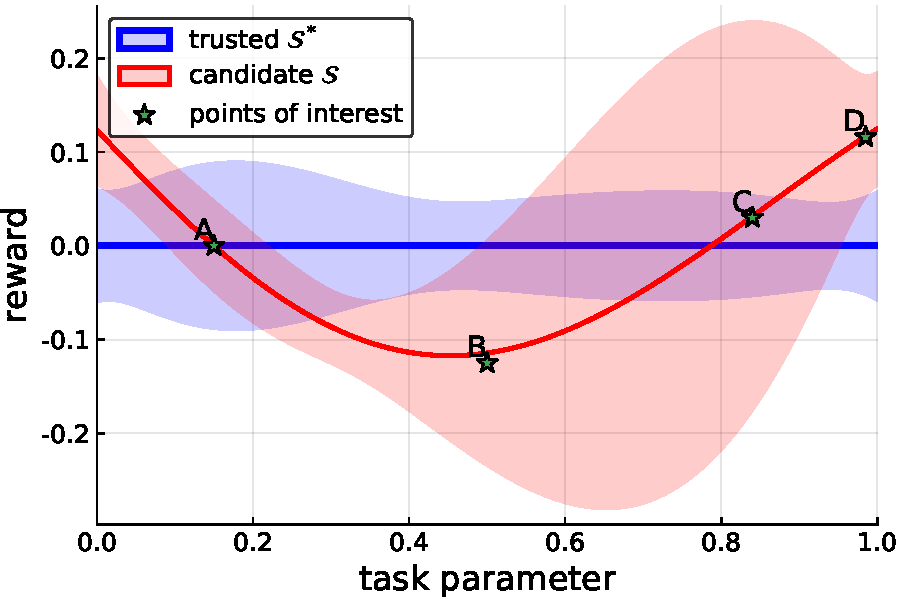
\includegraphics[width=1.0\linewidth]{Figures/p1.pdf}
        \vfill
        % \caption{tst}
        % \label{fig:}
    \end{subfigure}%
    \hfill
    \begin{subfigure}[t]{0.35\linewidth}
        \centering
        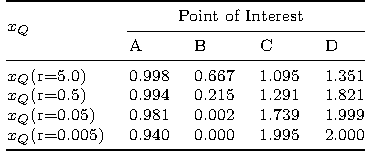
\includegraphics[width=1.0\linewidth]{Figures/p1_table.pdf}
        % \caption{Candidate solver depth 1}
        % \label{fig:med_roadnet}
    \end{subfigure} 
    \caption{Assessing \xQ{} calculation on reward fxn's: \solvestar{} (blue) and \solve{} (red). Points of interest indicated by a star.}
    \label{fig:sq_thry1}
\end{figure}
